\documentclass{article}
\newsavebox{\oldepsilon}
\savebox{\oldepsilon}{\ensuremath{\epsilon}}
\usepackage[minionint,mathlf,textlf]{MinionPro} % To gussy up a bit
\renewcommand*{\epsilon}{\usebox{\oldepsilon}}
\usepackage[margin=1in]{geometry}
\usepackage{graphicx} % For .eps inclusion
%\usepackage{indentfirst} % Controls indentation
\usepackage[compact]{titlesec} % For regulating spacing before section titles
\usepackage{adjustbox} % For vertically-aligned side-by-side minipages
\usepackage{array, amsmath,  mhchem}
\usepackage[hidelinks]{hyperref}
\usepackage{courier, subcaption}
\usepackage{multirow, enumerate}
\usepackage[autolinebreaks,framed,numbered]{mcode}
\usepackage{float}
\restylefloat{table}

\pagenumbering{gobble} 
\setlength\parindent{0 cm}
\renewcommand{\arraystretch}{1.2}
\begin{document}
\large

MCB 135 Problem Set 6 \hfill Due Wednesday, March 25, 2015 at 2:30 PM

\section*{Problem 1: Band pass filter (55 points)}

As many jet-setters discover, circadian clocks are not useful unless their phase is set appropriately. Entrainment is the process of setting a biological clock's phase in response to external cues such as sunlight. Unfortunately, entrainment cues themselves may be noisy and require filtering.\\

Consider an entrainment system whose input is the ambient light level $x(t)$, which oscillates with 24-hour period but is subject to many sources of variation. The system's output $y(t)$ would ideally be sinusoidal with period 24 hours and the same phase as the circadian signal.\\

\begin{center}
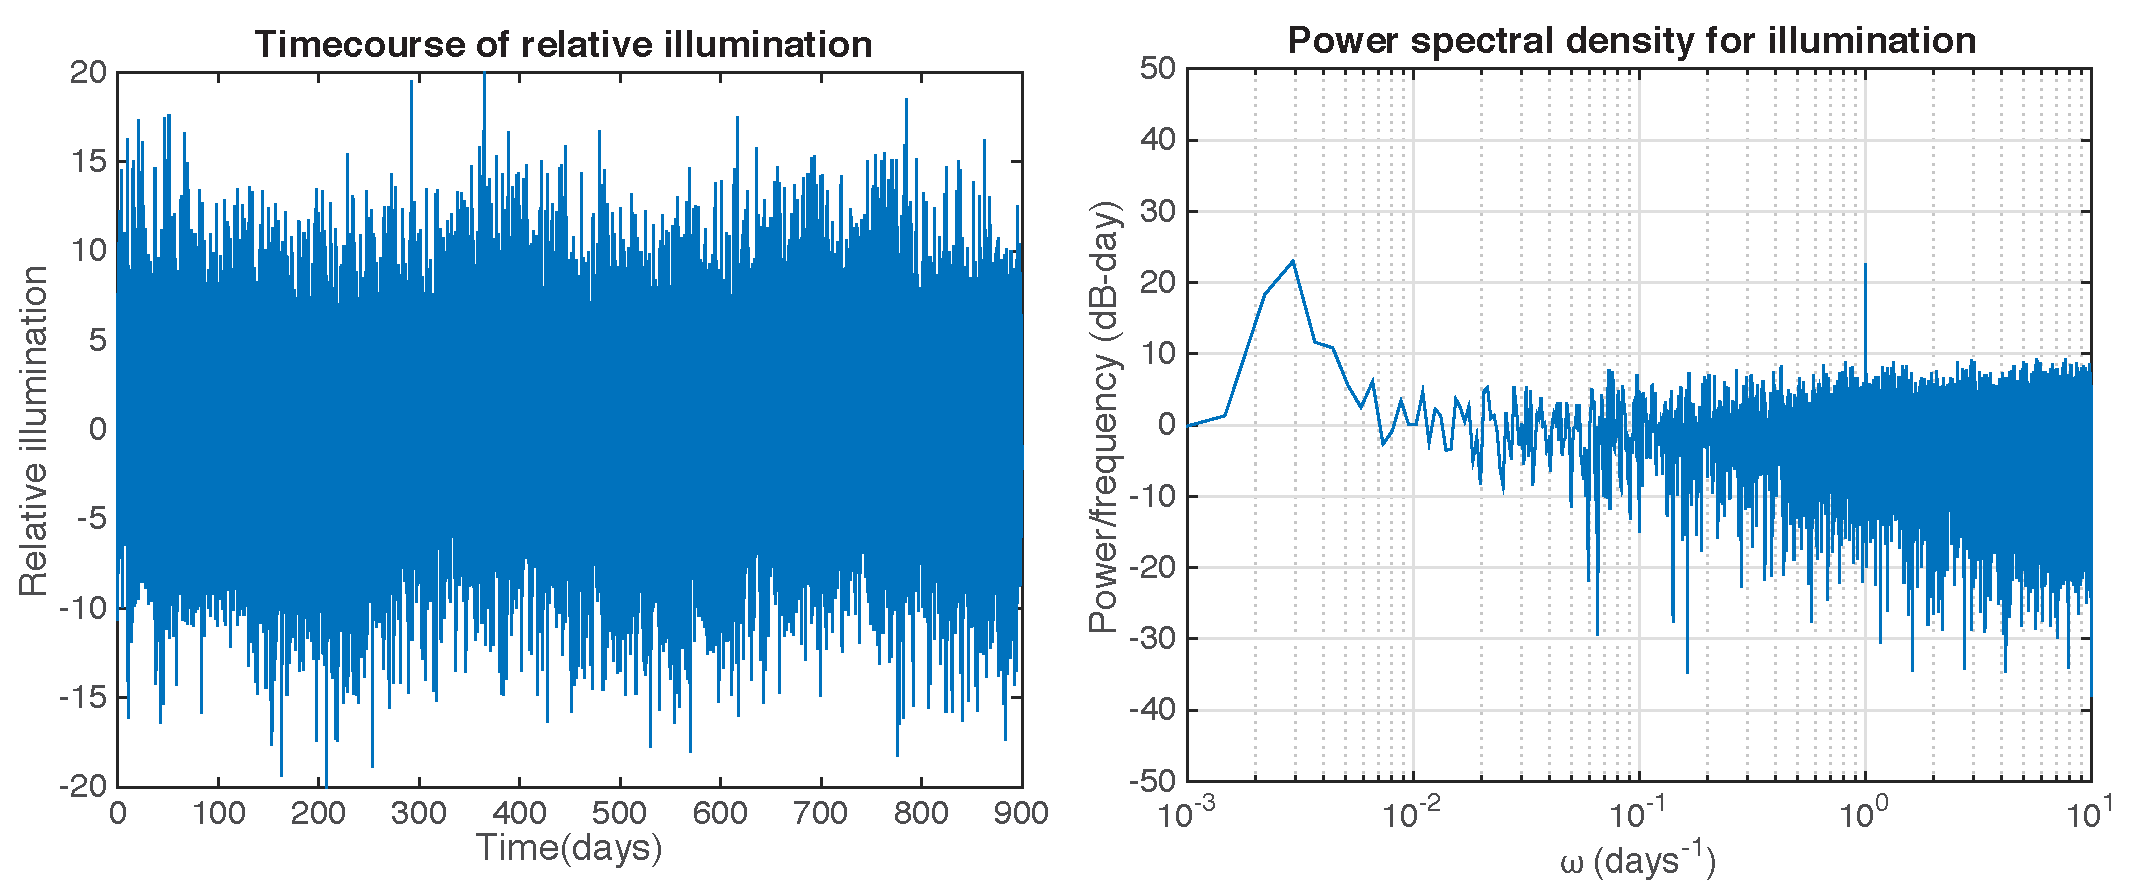
\includegraphics[width=.7\textwidth]{sun.pdf}
\end{center}

The time course at left shows $x(t)$ measurements taken every hour, beginning at noon, for 900 days. $x(t)$ was then decomposed into a combination of sine waves of different frequencies: the \textit{power spectral density }(PSD) plot at right gives the relative power of each wave vs. its frequency, $\omega$. The time course data and code used to generate the PSD are available on the course website.

\begin{enumerate}[a)]
\setlength{\itemsep}{0pt}
\item Which of the two major peaks in the PSD represents the signal we wish to amplify? What is the source of the other peak?\\

{\color{red}
The peak at $\omega = 1$ cycle per dayis the circadian signal which we wish to amplify. The second peak, with a frequency $\omega = 1$ cycle per 365 days is likely caused by annual fluctuations in average illumination.
}

\item Determine the closed loop transfer function for the system depicted below in terms of $K(s)$.

\begin{center}
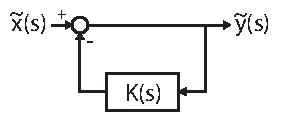
\includegraphics[width=.3\textwidth]{feedback.pdf}
\end{center}

{\color{red}
\begin{eqnarray*}
\tilde{y} & = & \left[ \tilde{x} - K(s) \tilde{y} \right] \\
\textrm{Closed loop transfer function } H(s) = \frac{\tilde{y}}{\tilde{x}} & = & \frac{1}{1+K(s)}
\end{eqnarray*}
}


\item What type of controller can be used to preferentially amplify high frequencies? Low frequencies?\\

{\color{red}
A derivative controller preferentially amplifies high frequencies, and an integral controller preferentially amplifies low frequencies.
}

\item Combine your answers in part (c) to choose a form for $K(s)$ so that the closed loop system filters out both high and low frequency noise. Include appropriate units on any constants\footnote{Hint: What is one period in radians? As you complete the remaining questions, it should become clear whether your units were selected properly.}.\\

{\color{red}
Choose $K(s) = \tau_d s + \frac{1}{\tau_i s}$ so that both high and low frequency noise are detected by the feedback loop and thus subtracted from the input signal; the closed loop transfer function is therefore:
\[ H(s) = \frac{s}{\tau_d s^2 + s + \frac{1}{\tau_i}} \]
The constants should be chosen so that there is no attenuation at the circadian signal's frequency ($\omega=1$ cycle per day = $2\pi$ radians per day). A trial-and-error approach to constant choice is acceptable; alternatively, we can calculate the magnitude of the closed loop transfer function at $\omega = 2\pi$ radians/day and find a relation on $\tau_d$ and $\tau_i$ from there:
\begin{eqnarray*}
1 = \left| H(s) \right|_{s=i\omega} & = &\left| \frac{i\omega}{-\tau_d \omega^2 + i \omega + \frac{1}{\tau_i}} \cdot \frac{-\tau_d \omega^2 - i \omega + \frac{1}{\tau_i}}{-\tau_d \omega^2 - i \omega + \frac{1}{\tau_i}} \right|\\
& = &  \left| \frac{\omega^2 + i\omega \left( -\tau_d \omega^2 + \frac{1}{\tau_i}\right)}{\omega^2 + \left( -\tau_d \omega^2 + \frac{1}{\tau_i}\right)^2} \right| = \frac{\omega \sqrt{\omega^2 + \left( -\tau_d \omega^2 + \frac{1}{\tau_i}\right)^2}}{\omega^2 + \left( -\tau_d \omega^2 + \frac{1}{\tau_i}\right)^2}\\
\sqrt{\omega^2 + \left( -\tau_d \omega^2 + \frac{1}{\tau_i}\right)^2} & = & \omega \implies \tau_d \tau_i = \frac{1}{\omega^2} = \frac{1}{4\pi^2} \textrm{ days$^2$ per radian$^2$}
\end{eqnarray*}
For example, we could choose $\tau_d = \frac{20}{2 \pi}$ days per radian and $\tau_i = \frac{1}{20 \times 2\pi}$ days per radian.
}

\item Construct a Bode plot for your closed loop system. Will the phase of the output be accurate for oscillations with a 24-hour period?\\

{\color{red}

All figures generated for this problem are included here for simplicity:

\begin{center}
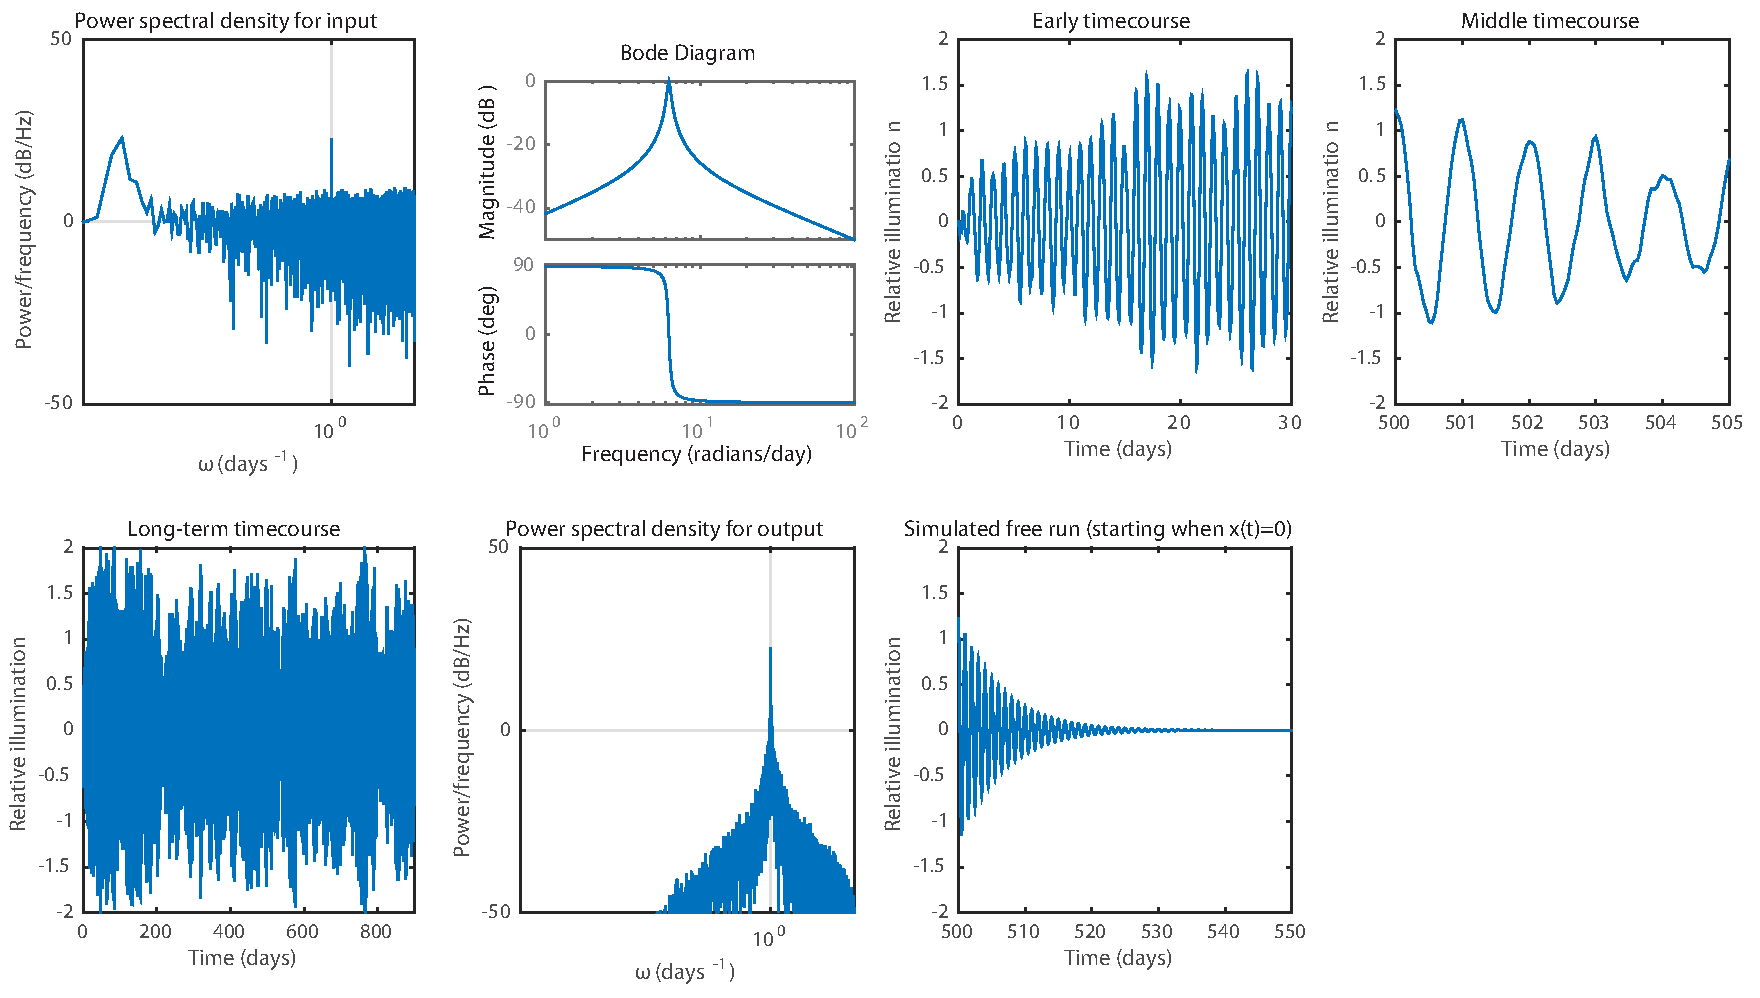
\includegraphics[width=\textwidth]{problem1figs.pdf}
\end{center}

The Bode plot for $H(s)$ (2nd from top left) shows the magnitude peak of 0 dB (1:1 ratio of input to output) at $\omega = 2\pi$ radians/day that we desired. At that frequency, the phase difference between input and output is zero, so we expect the phase of the output to accurately reflect the phase of the circadian signal.
}

\item Use MATLAB's \mcode{lsim()} function with the time course data and your closed loop transfer function to simulate the output of your system, $y(t)$. Include plots of $y(t)$ with appropriate windows to:
\begin{itemize}
\item Confirm that your system's output is dominated by oscillations with a 24-hour period.
\item Show the range of variation in amplitude over 900 days.
\item Indicate the ``burn-in" time, i.e., time elapsed before the system's output has reasonably steady phase and amplitude.
\end{itemize}

{\color{red}
See the early, middle, and long-term timecourses included in the composite figure above. The middle timecourse shows oscillations with a period of 1 day. The range in amplitude is shown in the long-term timecourse and seems to be a rather large spread. The early timecourse shows the slow initial increase in amplitude of the signal over the course of roughly 15-20 days: this is an estimate of the ``burn-in" time. (Note the relationship to our choice of $\tau_i$.)
}

\item Are there trade-offs between shorter burn-in time and variation in amplitude for the system you've designed? Demonstrate your conclusion by showing a plot with a different choice of parameters.\\

{\color{red}
For comparison, the following figure shows the results when we use $\tau_d=20$ and $\tau_i=\frac{1}{20(2\pi)^2}$ instead:

\begin{center}
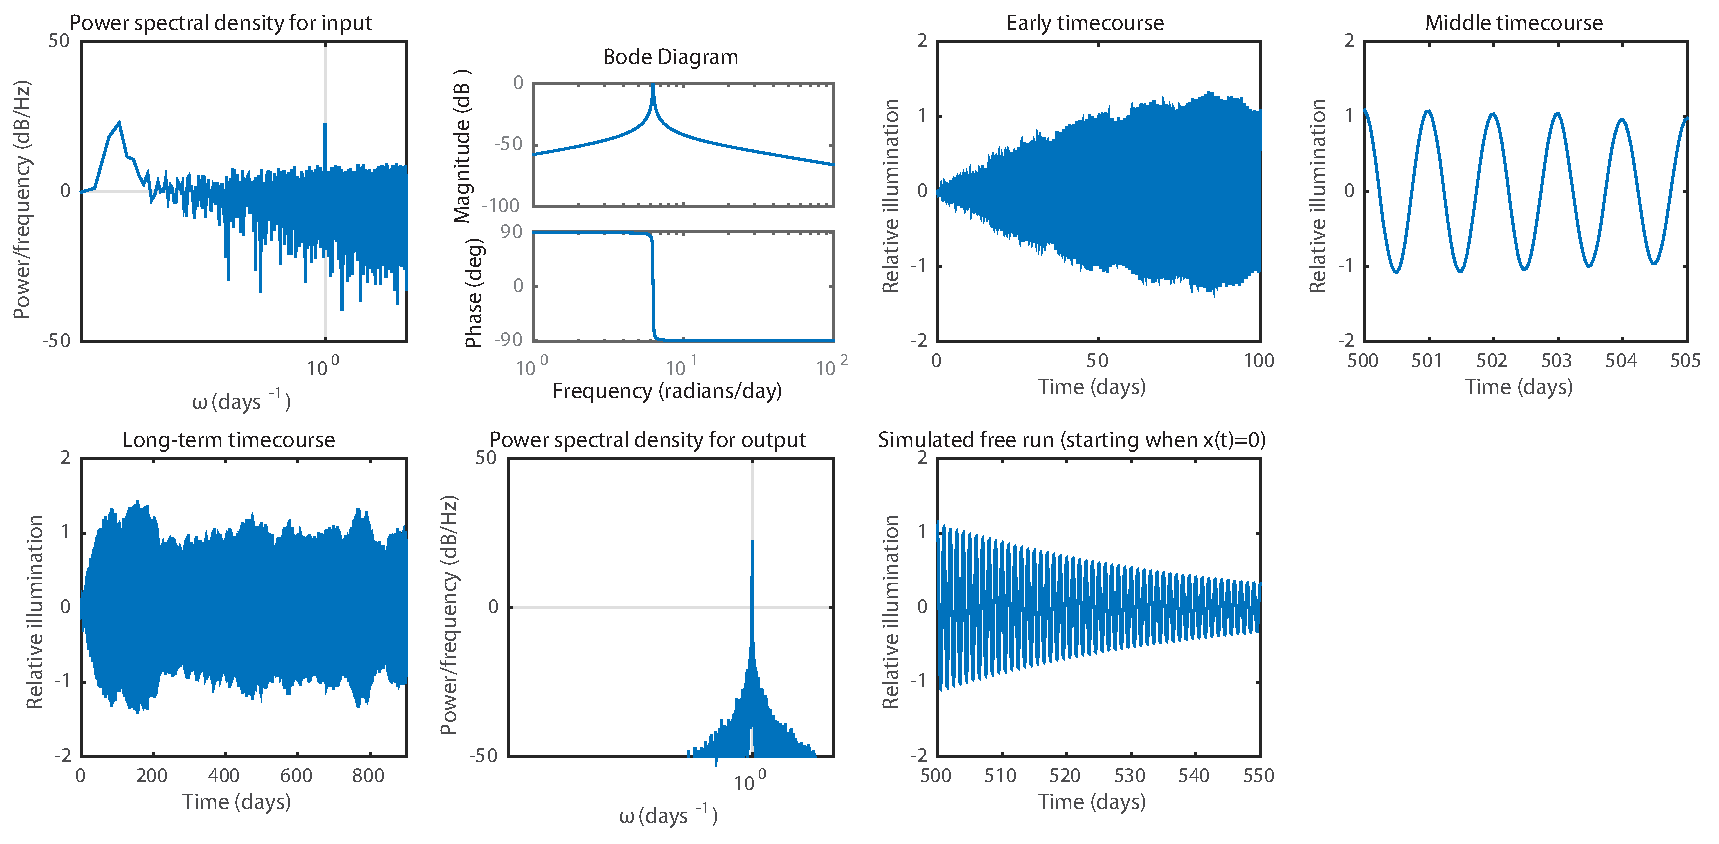
\includegraphics[width=\textwidth]{problem1figs2.pdf}
\end{center}

These constants give an output signal with greater uniformity in amplitude, but with a longer burn-in time of approximately 90-120 days. A general trade-off is expected between burn-in time and consistency in output signal amplitude because both depend on the choice of integral control time constant.
}

\item Simulate a ``free run" by setting $x(t)$ to zero at some time after the burn-in. How long does your system continue to oscillate appreciably?\\

{\color{red} The composite figures above show the result when we set $x(t)$ to zero for all times $t>500$ days. The length of time for which the system will continue to oscillate noticeably depends on the choice of constants used, e.g. about 20 days for the first example and about 120 days for the second example, as expected from the choice of $\tau_i$.\\

All code used in this problem appears below (an alternative transfer function used in problem 2 has been commented out):
}

\begin{lstlisting}
function [] = bode_timecourse_psd()
    % Load the data in from the file
    a = tdfread('illumination.tsv');
    t = a.x0';
    x = a.x70x2E58942367627401';

    % PSD for input (for your reference only)
    figure
    subplot(2,4,1)
    Fs = 24;
    nfft = 2^nextpow2(length(x));
    Pxx = abs(fft(x,nfft)).^2/length(x)/Fs;
    Hpsd2 = dspdata.psd(Pxx(1:length(Pxx)/2),'Fs',Fs);  
    plot(Hpsd2)
    axis([1E-3 10 -50 50])
    set(gca,'XScale','log')
    xlabel('\omega (days^{-1})')
    title('Power spectral density for input')
    
    % Bode plot for this transfer function
    % Resonator
    %gamma=0.001*2*pi;
    %k = 2*pi;
    %my_tf = tf([1 gamma],[1, 2*gamma, gamma^2 + k^2]);

    % Band pass
    tau_i = 1/(20*2*pi);
    tau_d = 20/(2*pi);
    my_tf = tf([1 0],[tau_d, 1, 1/tau_i]);
    
    subplot(2,4,2)
    bode(my_tf)
    xlabel('Frequency (radians/day)')
    
    % Simulate output
    y = lsim(my_tf,x,t);
    
    % Early timecourse (shows burn-in time)
    subplot(2,4,3)
    plot(t,y)
    axis([0 30 -2 2])
    title('Early timecourse')
    xlabel('Time (days)')
    ylabel('Relative illumination')
    
    % Middle timecourse (shows 24-hour oscillation and phase)
    subplot(2,4,4)
    plot(t,y)
    axis([500 505 -2 2])
    title('Middle timecourse')
    xlabel('Time (days)')
    ylabel('Relative illumination')
    
    % Full timecourse (shows variation in amplitude)
    subplot(2,4,5)
    plot(t,y)
    axis([0 900 -2 2])
    title('Long-term timecourse')
    xlabel('Time (days)')
    ylabel('Relative illumination')
    
    % PSD for output (for your reference only)
    subplot(2,4,6)
    Fs = 24;
    nfft = 2^nextpow2(length(y));
    Pyy = abs(fft(y,nfft)).^2/length(y)/Fs;
    Hpsd2 = dspdata.psd(Pyy(1:length(Pyy)/2),'Fs',Fs);  
    plot(Hpsd2)
    axis([1E-3 10 -50 50])
    set(gca,'XScale','log')
    xlabel('\omega (days^{-1})')
    title('Power spectral density for output')
    
    % Simulated free run -- input disappears at t=500 days
    x(24*500:end) = zeros(size(x(24*500:end)));
    y = lsim(my_tf,x,t);
    
    % Free run results
    subplot(2,4,7)
    plot(t,y)
    axis([500 550 -2 2])
    title('Simulated free run (starting when x(t)=0)')
    xlabel('Time (days)')
    ylabel('Relative illumination')
    
end
\end{lstlisting}
\end{enumerate}



\section*{Problem 2: Resonator (25 points)}

An alternative approach to amplify oscillations at a frequency of interest uses resonant systems. Consider the following system of two transcription factors, $A$ and $B$: expression of $A$ is driven by an input signal $x(t)$ but is repressed by $B$. $A$ activates expression of $B$. Both transcription factors are subject to dilution/degradation.

\begin{eqnarray*}
\frac{da}{dt} & = & x(t) - k b - \gamma a\\
\frac{db}{dt} & = & ka - \gamma b
\end{eqnarray*}

The output of this system is regarded to be the concentration $a(t)$.

\begin{enumerate}[a)]
\setlength{\itemsep}{0pt}
\item Apply a Laplace transformation to the system and rearrange to find the system's closed loop transfer function, $\frac{\tilde{a}(s)}{\tilde{x}(s)}$.\\

{\color{red} We will assume initial concentrations are zero to simply the transformation.
\begin{eqnarray*}
s\tilde{b} & = & k\tilde{a} - \gamma \tilde{b} \implies \tilde{b}  = \frac{k \tilde{a}}{s + \gamma}\\
s\tilde{a} & = & \tilde{x} - k\tilde{b} - \gamma \tilde{a} \implies \frac{\tilde{a}}{\tilde{x}} = \frac{1}{s + \gamma + \frac{k^2}{s+\gamma}} = \frac{s + \gamma}{s^2 + 2\gamma s + \gamma^2 + k^2}
\end{eqnarray*}
}

\item Prepare a Bode plot of this system with $\gamma=0.002 \pi $, $k=2\pi$.\\

{\color{red}
This figure was generated using the same code as above, with the transfer function for the resonator uncommented and some plotting bounds changed.

\begin{center}
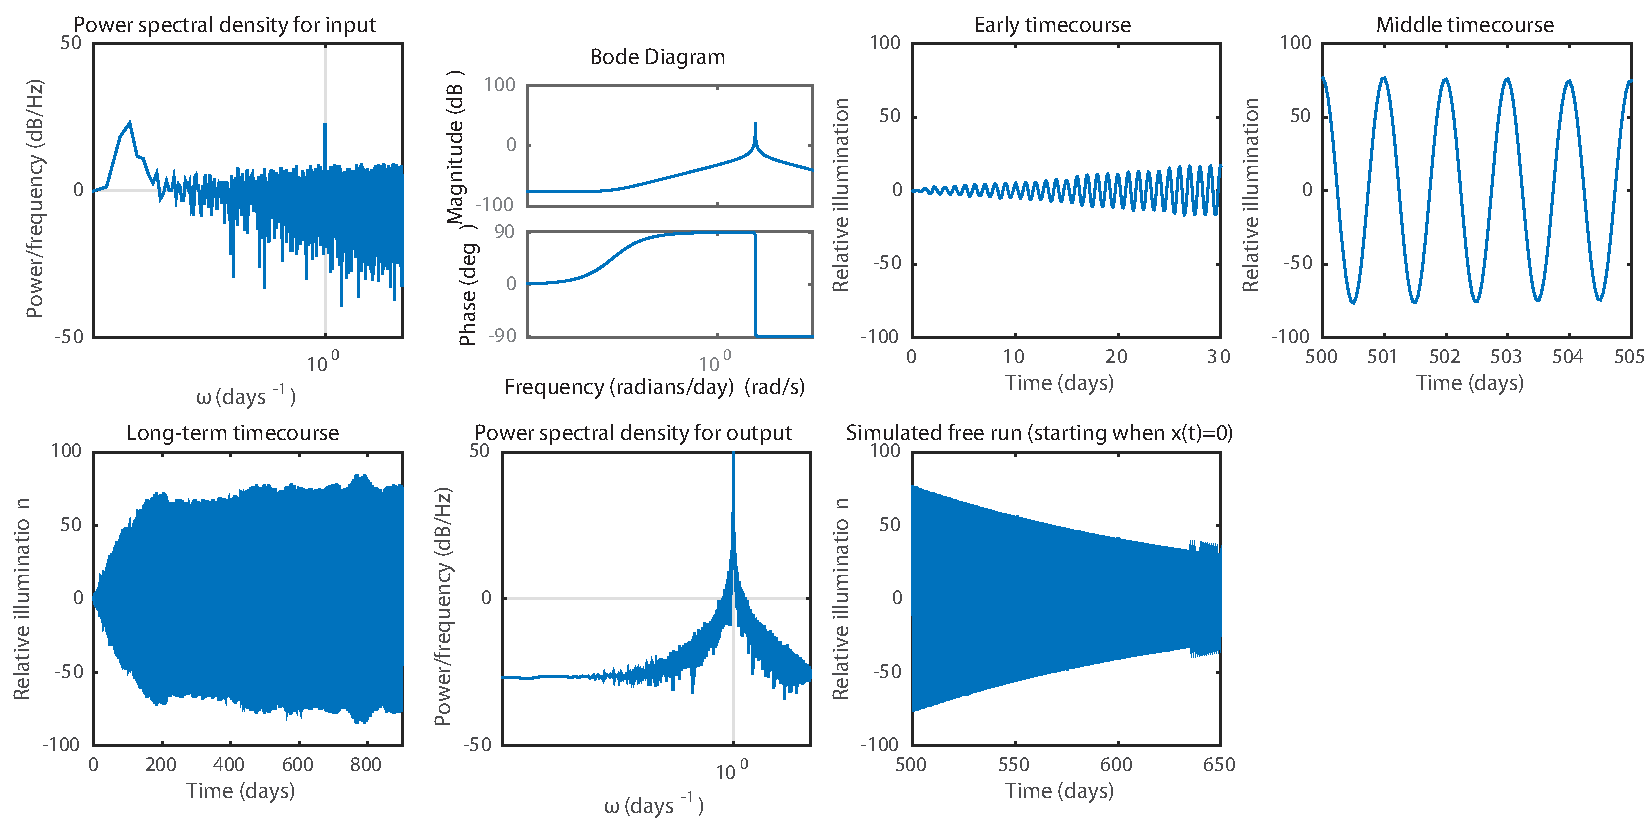
\includegraphics[width=\textwidth]{resonator.pdf}
\end{center}

}


\item Repeat problem 1f using the resonator transfer function. Compare the result to your band pass filter's output.\\

{\color{red}
The resonator performs comparably to the band pass filter with small integration constant: the burn-in time is long and the amplitude of the output is relatively consistent. One notable difference is that the circadian signal has been amplified, whereas the band pass filter merely avoided attenuating this signal.

}

\end{enumerate}

\section*{Problem 3: Alternative coherent feedforward loop (adapted from Alon 4.5, 20 points)}

\begin{minipage}[b]{0.1\linewidth}
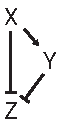
\includegraphics[width=\textwidth]{c3ffl.pdf}
\end{minipage}
\hspace{0.5cm}
\begin{minipage}[b]{0.85\linewidth}
Solve the dynamics of the type-3 coherent FFL (shown at left), assuming AND logic at the $Z$ promoter, in response to (i) a step increase and (ii) a step decrease in the concentration of $X$. Here, AND logic means that $Z$ is produced only if both $X$ and $Y$ are below their threshold concentrations for promoter binding. Are there delays? What logic gate does this circuit embody at steady-state? Compare your answers to the type-1 coherent FFL described in class.\\

\end{minipage}\\
{\color{red}
Define $K_X$ and $K_Y$ to be the threshold concentrations for activity of $X$ and $Y$.
\begin{eqnarray*}
\frac{dY}{dt} & = & \alpha_Y \Theta \left( X > K_ X \right) - \beta_Y Y\\ 
\frac{dZ}{dt} & = & \alpha_Z \Theta \left( X < K_ X \right) \Theta \left( Y < K_ Y \right) - \beta_Z Z
\end{eqnarray*}

\subsection*{Case one: $[X]<K_X \to [X] > K_X$}

We assume that prior to the step at $t=0$, the system has reached equilibrium with $X$ below its activity threshold: setting both time derivatives equal to zero, we find that $Y(0)=0$ and $Z(0) = \alpha_Z/\beta_Z$. After the step, $Y$ production immediately begins due to activation by $X$:
\[ \frac{dY(t \geq 0)}{dt} = \alpha_Y - \beta_Y Y \textrm{ and } Y(0) = 0  \implies Y(t \geq 0) = \frac{\alpha_Y}{\beta_Y} \left( 1 - e^{-\beta_Y t} \right) \]
After the step, $Z$ production immediately ceases due to repression by $X$:
\[ \frac{dZ(t \geq 0)}{dt} = - \beta_Z Z \textrm{ and } Z(0) = \frac{\alpha_Z}{\beta_Z} \implies Z(t \geq 0) = \frac{\alpha_Z}{\beta_Z} e^{-\beta_Z t} \]

\subsection*{Case two: $[X]>K_X \to [X] < K_X$}

We assume that prior to the step at $t=0$, the system has reached equilibrium with $X$ above its activity threshold: setting both time derivatives equal to zero, we find that $Y(0)=\alpha_Y/\beta_Y$ and $Z(0) = 0$. After the step, $Y$ production immediately ceases due to loss of activation by $X$:
\[ \frac{dY(t \geq 0)}{dt} = - \beta_Y Y \textrm{ and } Y(0) = \frac{\alpha_Y}{\beta_Y}  \implies Y(t \geq 0) = \frac{\alpha_Y}{\beta_Y} e^{-\beta_Y t} \]
In particular, $Y$ will fall below its activity threshold at time $\tau$:
\[ \frac{\alpha_Y}{\beta_Y} e^{-\beta_Y t} = \tau \implies \tau = \frac{1}{\beta_Y} \ln \left( \frac{\alpha_Y}{\beta_Y K_Y} \right) \]
$Z$ production commences at time $\tau$ when repression by both $X$ and $Y$ has lifted:
\[ \frac{dZ(t \geq \tau)}{dt} = \alpha_Z - \beta_Z Z \textrm{ and } Z(0) = Z(\tau) = 0 \implies Z(t \geq \tau) = \frac{\alpha_Z}{\beta_Z} \left( 1 - e^{-\beta_Z (t-\tau)} \right) \]

\subsection*{Summary and comparison}

The C3-FFL with AND logic has a time delay only for the ``off" step, whereas the C1-FFL with AND logic has a time delay only for the ``on" step. Furthermore, the C3-FFL implements ``NOT X" logic at steady state: by comparison, the C1-FFL implements ``X" logic at steady state.

}




\end{document}